\documentclass{standalone}
\usepackage{tikz}
\usetikzlibrary{patterns, positioning}


\begin{document}
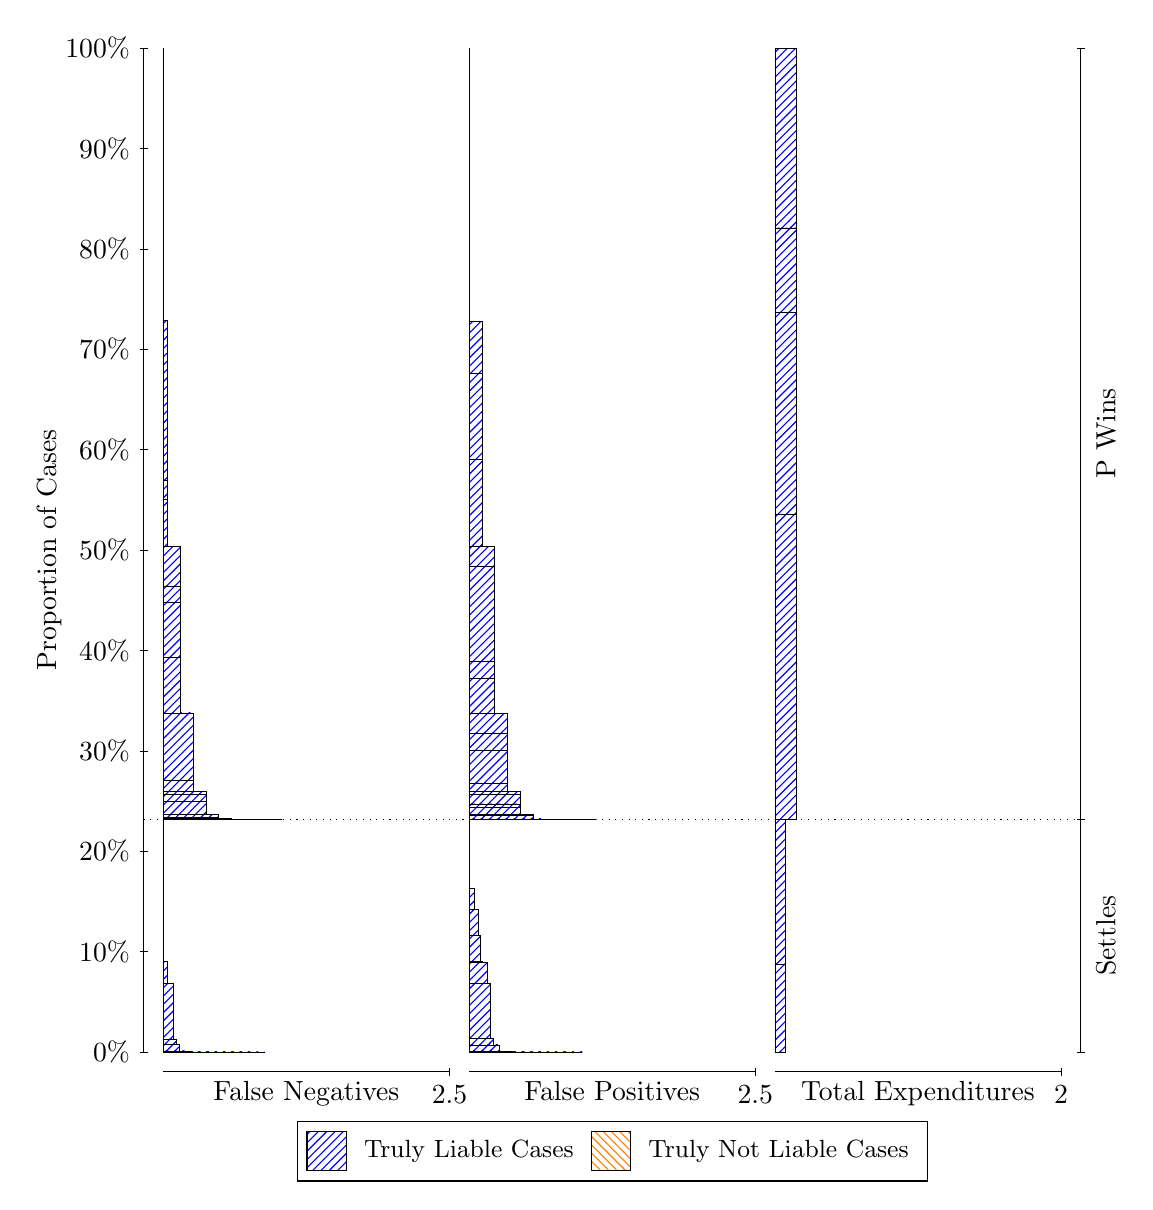
\begin{tikzpicture}
\draw[black, very thin] (1.5,1.75) -- (1.5,14.5);
\node[rotate=90, text=black, anchor=center] at (0.3, 8.125) {Proportion of Cases};
\draw[black, very thin] (1.45,1.75) -- (1.55,1.75);
\node[text=black, anchor=east] at (1.45, 1.75) {0\%};
\draw[black, very thin] (1.45,3.025) -- (1.55,3.025);
\node[text=black, anchor=east] at (1.45, 3.025) {10\%};
\draw[black, very thin] (1.45,4.3) -- (1.55,4.3);
\node[text=black, anchor=east] at (1.45, 4.3) {20\%};
\draw[black, very thin] (1.45,5.575) -- (1.55,5.575);
\node[text=black, anchor=east] at (1.45, 5.575) {30\%};
\draw[black, very thin] (1.45,6.85) -- (1.55,6.85);
\node[text=black, anchor=east] at (1.45, 6.85) {40\%};
\draw[black, very thin] (1.45,8.125) -- (1.55,8.125);
\node[text=black, anchor=east] at (1.45, 8.125) {50\%};
\draw[black, very thin] (1.45,9.4) -- (1.55,9.4);
\node[text=black, anchor=east] at (1.45, 9.4) {60\%};
\draw[black, very thin] (1.45,10.675) -- (1.55,10.675);
\node[text=black, anchor=east] at (1.45, 10.675) {70\%};
\draw[black, very thin] (1.45,11.95) -- (1.55,11.95);
\node[text=black, anchor=east] at (1.45, 11.95) {80\%};
\draw[black, very thin] (1.45,13.225) -- (1.55,13.225);
\node[text=black, anchor=east] at (1.45, 13.225) {90\%};
\draw[black, very thin] (1.45,14.5) -- (1.55,14.5);
\node[text=black, anchor=east] at (1.45, 14.5) {100\%};

\draw[black, very thin] (13.4,1.75) -- (13.4,14.5);
\draw[black, very thin] (13.35,1.75) -- (13.45,1.75);
\node[anchor=west] at (13.35, 1.75) {};
\draw[black, very thin] (13.35,4.7043) -- (13.45,4.7043);
\node[anchor=west] at (13.35, 4.7043) {};
\draw[black, very thin] (13.35,14.5) -- (13.45,14.5);
\node[anchor=west] at (13.35, 14.5) {};

\draw[black, very thin, pattern color=blue, pattern=north east lines] (1.75,1.75) rectangle (3.0398,1.75);
\draw[black, very thin, pattern color=blue, pattern=north east lines] (1.75,1.75) rectangle (2.8784,1.75);
\draw[black, very thin, pattern color=blue, pattern=north east lines] (1.75,1.75) rectangle (2.8218,1.75);
\draw[black, very thin, pattern color=blue, pattern=north east lines] (1.75,1.75) rectangle (2.7169,1.75);
\draw[black, very thin, pattern color=blue, pattern=north east lines] (1.75,1.75) rectangle (2.6604,1.75);
\draw[black, very thin, pattern color=blue, pattern=north east lines] (1.75,1.75) rectangle (2.6038,1.75);
\draw[black, very thin, pattern color=blue, pattern=north east lines] (1.75,1.75) rectangle (2.5554,1.75);
\draw[black, very thin, pattern color=blue, pattern=north east lines] (1.75,1.75) rectangle (2.4989,1.75);
\draw[black, very thin, pattern color=blue, pattern=north east lines] (1.75,1.75) rectangle (2.4585,1.75);
\draw[black, very thin, pattern color=blue, pattern=north east lines] (1.75,1.75) rectangle (2.4424,1.75);
\draw[black, very thin, pattern color=blue, pattern=north east lines] (1.75,1.75) rectangle (2.3939,1.75);
\draw[black, very thin, pattern color=blue, pattern=north east lines] (1.75,1.75) rectangle (2.3374,1.75);
\draw[black, very thin, pattern color=blue, pattern=north east lines] (1.75,1.75) rectangle (2.297,1.75);
\draw[black, very thin, pattern color=blue, pattern=north east lines] (1.75,1.75) rectangle (2.2809,1.7503);
\draw[black, very thin, pattern color=blue, pattern=north east lines] (1.75,1.7503) rectangle (2.2405,1.7503);
\draw[black, very thin, pattern color=blue, pattern=north east lines] (1.75,1.7503) rectangle (2.2324,1.7504);
\draw[black, very thin, pattern color=blue, pattern=north east lines] (1.75,1.7504) rectangle (2.1759,1.7504);
\draw[black, very thin, pattern color=blue, pattern=north east lines] (1.75,1.7504) rectangle (2.1355,1.7504);
\draw[black, very thin, pattern color=blue, pattern=north east lines] (1.75,1.7504) rectangle (2.1194,1.7582);
\draw[black, very thin, pattern color=blue, pattern=north east lines] (1.75,1.7582) rectangle (2.079,1.7582);
\draw[black, very thin, pattern color=blue, pattern=north east lines] (1.75,1.7582) rectangle (2.0709,1.7635);
\draw[black, very thin, pattern color=blue, pattern=north east lines] (1.75,1.7635) rectangle (2.0144,1.7637);
\draw[black, very thin, pattern color=blue, pattern=north east lines] (1.75,1.7637) rectangle (1.9741,1.7637);
\draw[black, very thin, pattern color=blue, pattern=north east lines] (1.75,1.7637) rectangle (1.9579,1.8431);
\draw[black, very thin, pattern color=blue, pattern=north east lines] (1.75,1.8431) rectangle (1.9175,1.8432);
\draw[black, very thin, pattern color=blue, pattern=north east lines] (1.75,1.8432) rectangle (1.9095,1.9157);
\draw[black, very thin, pattern color=blue, pattern=north east lines] (1.75,1.9157) rectangle (1.8772,2.6218);
\draw[black, very thin, pattern color=blue, pattern=north east lines] (1.75,2.6218) rectangle (1.8529,2.6241);
\draw[black, very thin, pattern color=blue, pattern=north east lines] (1.75,2.6241) rectangle (1.8126,2.6241);
\draw[black, very thin, pattern color=blue, pattern=north east lines] (1.75,2.6241) rectangle (1.7964,2.8959);
\draw[black, very thin, pattern color=blue, pattern=north east lines] (1.75,2.8959) rectangle (1.7561,2.896);
\draw[black, very thin, pattern color=orange, pattern=north west lines] (1.75,2.896) rectangle (1.75,2.896);
\draw[black, very thin, pattern color=blue, pattern=north east lines] (1.75,2.896) rectangle (1.75,4.7043);
\draw[black, very thin, pattern color=blue, pattern=north east lines] (1.75,4.7043) rectangle (3.2578,4.7043);
\draw[black, very thin, pattern color=blue, pattern=north east lines] (1.75,4.7043) rectangle (3.0964,4.7043);
\draw[black, very thin, pattern color=blue, pattern=north east lines] (1.75,4.7043) rectangle (3.0964,4.7043);
\draw[black, very thin, pattern color=blue, pattern=north east lines] (1.75,4.7043) rectangle (2.9349,4.7043);
\draw[black, very thin, pattern color=blue, pattern=north east lines] (1.75,4.7043) rectangle (2.7734,4.7045);
\draw[black, very thin, pattern color=blue, pattern=north east lines] (1.75,4.7045) rectangle (2.7734,4.7048);
\draw[black, very thin, pattern color=blue, pattern=north east lines] (1.75,4.7048) rectangle (2.6119,4.7105);
\draw[black, very thin, pattern color=blue, pattern=north east lines] (1.75,4.7105) rectangle (2.6119,4.7119);
\draw[black, very thin, pattern color=blue, pattern=north east lines] (1.75,4.7119) rectangle (2.4504,4.722);
\draw[black, very thin, pattern color=blue, pattern=north east lines] (1.75,4.722) rectangle (2.4504,4.7327);
\draw[black, very thin, pattern color=blue, pattern=north east lines] (1.75,4.7327) rectangle (2.4504,4.7691);
\draw[black, very thin, pattern color=blue, pattern=north east lines] (1.75,4.7691) rectangle (2.2889,4.9347);
\draw[black, very thin, pattern color=blue, pattern=north east lines] (1.75,4.9347) rectangle (2.2889,5.0212);
\draw[black, very thin, pattern color=blue, pattern=north east lines] (1.75,5.0212) rectangle (2.2889,5.0639);
\draw[black, very thin, pattern color=blue, pattern=north east lines] (1.75,5.0639) rectangle (2.1275,5.1966);
\draw[black, very thin, pattern color=blue, pattern=north east lines] (1.75,5.1966) rectangle (2.1275,6.0552);
\draw[black, very thin, pattern color=blue, pattern=north east lines] (1.75,6.0552) rectangle (1.966,6.7627);
\draw[black, very thin, pattern color=blue, pattern=north east lines] (1.75,6.7627) rectangle (1.966,7.4587);
\draw[black, very thin, pattern color=blue, pattern=north east lines] (1.75,7.4587) rectangle (1.966,7.6704);
\draw[black, very thin, pattern color=blue, pattern=north east lines] (1.75,7.6704) rectangle (1.966,8.1752);
\draw[black, very thin, pattern color=blue, pattern=north east lines] (1.75,8.1752) rectangle (1.8045,8.7743);
\draw[black, very thin, pattern color=blue, pattern=north east lines] (1.75,8.7743) rectangle (1.8045,9.0098);
\draw[black, very thin, pattern color=blue, pattern=north east lines] (1.75,9.0098) rectangle (1.8045,11.037);
\draw[black, very thin, pattern color=orange, pattern=north west lines] (1.75,11.037) rectangle (1.75,11.037);
\draw[black, very thin, pattern color=blue, pattern=north east lines] (1.75,11.037) rectangle (1.75,14.5);
\draw[black, very thin, pattern color=orange, pattern=north west lines] (5.6333,1.75) rectangle (7.0685,1.75);
\draw[black, very thin, pattern color=blue, pattern=north east lines] (5.6333,1.75) rectangle (7.0685,1.75);
\draw[black, very thin, pattern color=blue, pattern=north east lines] (5.6333,1.75) rectangle (6.907,1.75);
\draw[black, very thin, pattern color=blue, pattern=north east lines] (5.6333,1.75) rectangle (6.7455,1.75);
\draw[black, very thin, pattern color=orange, pattern=north west lines] (5.6333,1.75) rectangle (6.7052,1.75);
\draw[black, very thin, pattern color=blue, pattern=north east lines] (5.6333,1.75) rectangle (6.7052,1.75);
\draw[black, very thin, pattern color=blue, pattern=north east lines] (5.6333,1.75) rectangle (6.5841,1.75);
\draw[black, very thin, pattern color=blue, pattern=north east lines] (5.6333,1.75) rectangle (6.5437,1.75);
\draw[black, very thin, pattern color=orange, pattern=north west lines] (5.6333,1.75) rectangle (6.4872,1.75);
\draw[black, very thin, pattern color=blue, pattern=north east lines] (5.6333,1.75) rectangle (6.4872,1.75);
\draw[black, very thin, pattern color=blue, pattern=north east lines] (5.6333,1.75) rectangle (6.4226,1.75);
\draw[black, very thin, pattern color=blue, pattern=north east lines] (5.6333,1.75) rectangle (6.3822,1.75);
\draw[black, very thin, pattern color=orange, pattern=north west lines] (5.6333,1.75) rectangle (6.3418,1.75);
\draw[black, very thin, pattern color=blue, pattern=north east lines] (5.6333,1.75) rectangle (6.3418,1.7502);
\draw[black, very thin, pattern color=blue, pattern=north east lines] (5.6333,1.7502) rectangle (6.3257,1.7502);
\draw[black, very thin, pattern color=blue, pattern=north east lines] (5.6333,1.7502) rectangle (6.2611,1.7505);
\draw[black, very thin, pattern color=blue, pattern=north east lines] (5.6333,1.7505) rectangle (6.2207,1.7505);
\draw[black, very thin, pattern color=blue, pattern=north east lines] (5.6333,1.7505) rectangle (6.1804,1.7567);
\draw[black, very thin, pattern color=blue, pattern=north east lines] (5.6333,1.7567) rectangle (6.1642,1.7567);
\draw[black, very thin, pattern color=orange, pattern=north west lines] (5.6333,1.7567) rectangle (6.1238,1.7567);
\draw[black, very thin, pattern color=blue, pattern=north east lines] (5.6333,1.7567) rectangle (6.1238,1.7569);
\draw[black, very thin, pattern color=blue, pattern=north east lines] (5.6333,1.7569) rectangle (6.0996,1.7645);
\draw[black, very thin, pattern color=blue, pattern=north east lines] (5.6333,1.7645) rectangle (6.0592,1.7645);
\draw[black, very thin, pattern color=blue, pattern=north east lines] (5.6333,1.7645) rectangle (6.0189,1.8392);
\draw[black, very thin, pattern color=blue, pattern=north east lines] (5.6333,1.8392) rectangle (6.0027,1.8392);
\draw[black, very thin, pattern color=blue, pattern=north east lines] (5.6333,1.8392) rectangle (5.9624,1.8414);
\draw[black, very thin, pattern color=blue, pattern=north east lines] (5.6333,1.8414) rectangle (5.9381,1.9191);
\draw[black, very thin, pattern color=orange, pattern=north west lines] (5.6333,1.9191) rectangle (5.9058,1.9191);
\draw[black, very thin, pattern color=blue, pattern=north east lines] (5.6333,1.9191) rectangle (5.9058,2.625);
\draw[black, very thin, pattern color=blue, pattern=north east lines] (5.6333,2.625) rectangle (5.8978,2.625);
\draw[black, very thin, pattern color=blue, pattern=north east lines] (5.6333,2.625) rectangle (5.8574,2.8947);
\draw[black, very thin, pattern color=blue, pattern=north east lines] (5.6333,2.8947) rectangle (5.8412,2.8947);
\draw[black, very thin, pattern color=blue, pattern=north east lines] (5.6333,2.8947) rectangle (5.8009,2.8999);
\draw[black, very thin, pattern color=blue, pattern=north east lines] (5.6333,2.8999) rectangle (5.7766,3.2302);
\draw[black, very thin, pattern color=blue, pattern=north east lines] (5.6333,3.2302) rectangle (5.7444,3.5583);
\draw[black, very thin, pattern color=blue, pattern=north east lines] (5.6333,3.5583) rectangle (5.7363,3.5583);
\draw[black, very thin, pattern color=blue, pattern=north east lines] (5.6333,3.5583) rectangle (5.6959,3.8302);
\draw[black, very thin, pattern color=blue, pattern=north east lines] (5.6333,3.8302) rectangle (5.6798,3.8302);
\draw[black, very thin, pattern color=blue, pattern=north east lines] (5.6333,3.8302) rectangle (5.6394,3.8325);
\draw[black, very thin, pattern color=blue, pattern=north east lines] (5.6333,3.8325) rectangle (5.6333,4.7043);
\draw[black, very thin, pattern color=orange, pattern=north west lines] (5.6333,4.7043) rectangle (7.2502,4.7043);
\draw[black, very thin, pattern color=blue, pattern=north east lines] (5.6333,4.7043) rectangle (7.2502,4.7043);
\draw[black, very thin, pattern color=orange, pattern=north west lines] (5.6333,4.7043) rectangle (7.0887,4.7043);
\draw[black, very thin, pattern color=blue, pattern=north east lines] (5.6333,4.7043) rectangle (7.0887,4.7043);
\draw[black, very thin, pattern color=blue, pattern=north east lines] (5.6333,4.7043) rectangle (6.9272,4.7043);
\draw[black, very thin, pattern color=orange, pattern=north west lines] (5.6333,4.7043) rectangle (6.9272,4.7043);
\draw[black, very thin, pattern color=blue, pattern=north east lines] (5.6333,4.7043) rectangle (6.9272,4.7043);
\draw[black, very thin, pattern color=blue, pattern=north east lines] (5.6333,4.7043) rectangle (6.7657,4.7044);
\draw[black, very thin, pattern color=blue, pattern=north east lines] (5.6333,4.7044) rectangle (6.7657,4.7046);
\draw[black, very thin, pattern color=orange, pattern=north west lines] (5.6333,4.7046) rectangle (6.7657,4.7046);
\draw[black, very thin, pattern color=blue, pattern=north east lines] (5.6333,4.7046) rectangle (6.7657,4.7048);
\draw[black, very thin, pattern color=orange, pattern=north west lines] (5.6333,4.7048) rectangle (6.6042,4.7048);
\draw[black, very thin, pattern color=blue, pattern=north east lines] (5.6333,4.7048) rectangle (6.6042,4.7084);
\draw[black, very thin, pattern color=blue, pattern=north east lines] (5.6333,4.7084) rectangle (6.6042,4.7098);
\draw[black, very thin, pattern color=blue, pattern=north east lines] (5.6333,4.7098) rectangle (6.6042,4.7112);
\draw[black, very thin, pattern color=orange, pattern=north west lines] (5.6333,4.7112) rectangle (6.4428,4.7112);
\draw[black, very thin, pattern color=blue, pattern=north east lines] (5.6333,4.7112) rectangle (6.4428,4.7554);
\draw[black, very thin, pattern color=blue, pattern=north east lines] (5.6333,4.7554) rectangle (6.4428,4.7654);
\draw[black, very thin, pattern color=blue, pattern=north east lines] (5.6333,4.7654) rectangle (6.2813,4.8585);
\draw[black, very thin, pattern color=blue, pattern=north east lines] (5.6333,4.8585) rectangle (6.2813,4.9008);
\draw[black, very thin, pattern color=orange, pattern=north west lines] (5.6333,4.9008) rectangle (6.2813,4.9008);
\draw[black, very thin, pattern color=blue, pattern=north east lines] (5.6333,4.9008) rectangle (6.2813,5.0187);
\draw[black, very thin, pattern color=blue, pattern=north east lines] (5.6333,5.0187) rectangle (6.2813,5.0569);
\draw[black, very thin, pattern color=blue, pattern=north east lines] (5.6333,5.0569) rectangle (6.1198,5.1687);
\draw[black, very thin, pattern color=blue, pattern=north east lines] (5.6333,5.1687) rectangle (6.1198,5.5797);
\draw[black, very thin, pattern color=orange, pattern=north west lines] (5.6333,5.5797) rectangle (6.1198,5.5797);
\draw[black, very thin, pattern color=blue, pattern=north east lines] (5.6333,5.5797) rectangle (6.1198,5.8034);
\draw[black, very thin, pattern color=blue, pattern=north east lines] (5.6333,5.8034) rectangle (6.1198,6.0475);
\draw[black, very thin, pattern color=blue, pattern=north east lines] (5.6333,6.0475) rectangle (5.9583,6.4958);
\draw[black, very thin, pattern color=blue, pattern=north east lines] (5.6333,6.4958) rectangle (5.9583,6.7082);
\draw[black, very thin, pattern color=orange, pattern=north west lines] (5.6333,6.7082) rectangle (5.9583,6.7082);
\draw[black, very thin, pattern color=blue, pattern=north east lines] (5.6333,6.7082) rectangle (5.9583,7.9151);
\draw[black, very thin, pattern color=blue, pattern=north east lines] (5.6333,7.9151) rectangle (5.9583,8.1674);
\draw[black, very thin, pattern color=blue, pattern=north east lines] (5.6333,8.1674) rectangle (5.7968,9.271);
\draw[black, very thin, pattern color=orange, pattern=north west lines] (5.6333,9.271) rectangle (5.7968,9.271);
\draw[black, very thin, pattern color=blue, pattern=north east lines] (5.6333,9.271) rectangle (5.7968,10.369);
\draw[black, very thin, pattern color=blue, pattern=north east lines] (5.6333,10.369) rectangle (5.7968,11.029);
\draw[black, very thin, pattern color=blue, pattern=north east lines] (5.6333,11.029) rectangle (5.6354,11.297);
\draw[black, very thin, pattern color=blue, pattern=north east lines] (5.6333,11.297) rectangle (5.6354,12.884);
\draw[black, very thin, pattern color=blue, pattern=north east lines] (5.6333,12.884) rectangle (5.6354,13.149);
\draw[black, very thin, pattern color=blue, pattern=north east lines] (5.6333,13.149) rectangle (5.6333,14.5);
\draw[black, very thin, pattern color=orange, pattern=north west lines] (9.5167,1.75) rectangle (9.6529,1.75);
\draw[black, very thin, pattern color=blue, pattern=north east lines] (9.5167,1.75) rectangle (9.6529,2.8618);
\draw[black, very thin, pattern color=orange, pattern=north west lines] (9.5167,2.8618) rectangle (9.6529,2.8618);
\draw[black, very thin, pattern color=blue, pattern=north east lines] (9.5167,2.8618) rectangle (9.6529,4.7043);
\draw[black, very thin, pattern color=orange, pattern=north west lines] (9.5167,4.7043) rectangle (9.7892,4.7043);
\draw[black, very thin, pattern color=blue, pattern=north east lines] (9.5167,4.7043) rectangle (9.7892,8.5765);
\draw[black, very thin, pattern color=orange, pattern=north west lines] (9.5167,8.5765) rectangle (9.7892,8.5765);
\draw[black, very thin, pattern color=blue, pattern=north east lines] (9.5167,8.5765) rectangle (9.7892,11.142);
\draw[black, very thin, pattern color=orange, pattern=north west lines] (9.5167,11.142) rectangle (9.7892,11.142);
\draw[black, very thin, pattern color=blue, pattern=north east lines] (9.5167,11.142) rectangle (9.7892,12.217);
\draw[black, very thin, pattern color=orange, pattern=north west lines] (9.5167,12.217) rectangle (9.7892,12.217);
\draw[black, very thin, pattern color=blue, pattern=north east lines] (9.5167,12.217) rectangle (9.7892,14.5);
\draw[black, dotted] (1.5,4.7043) -- (13.4,4.7043);
\draw[black, very thin] (1.75,1.5) -- (5.3833,1.5);
\node[text=black, anchor=north] at (3.5667, 1.5) {False Negatives};
\draw[black, very thin] (5.3833,1.45) -- (5.3833,1.55);
\node[text=black, anchor=north] at (5.3833, 1.45) {2.5};

\draw[black, very thin] (5.6333,1.5) -- (9.2667,1.5);
\node[text=black, anchor=north] at (7.45, 1.5) {False Positives};
\draw[black, very thin] (9.2667,1.45) -- (9.2667,1.55);
\node[text=black, anchor=north] at (9.2667, 1.45) {2.5};

\draw[black, very thin] (9.5167,1.5) -- (13.15,1.5);
\node[text=black, anchor=north] at (11.333, 1.5) {Total Expenditures};
\draw[black, very thin] (13.15,1.45) -- (13.15,1.55);
\node[text=black, anchor=north] at (13.15, 1.45) {2};

\node[text=black, centered, rotate=90] at (13.72, 3.2271) {Settles};
\node[text=black, centered, rotate=90] at (13.72, 9.6021) {P Wins};

\draw (7.449999999999999,1.5) node[draw=none] (baseCoordinate) {};
\begin{scope}[align=center]
        \matrix[scale=0.5, draw=black, below=0.5cm of baseCoordinate, nodes={draw}, column sep=0.1cm]{
            \node[rectangle, draw, minimum width=0.5cm, minimum height=0.5cm, pattern color=blue, pattern=north east lines] {}; &
            \node[draw=none, font=\small, text=black] (B) {Truly Liable Cases}; &
            \node[rectangle, draw, minimum width=0.5cm, minimum height=0.5cm, pattern color=orange, pattern=north west lines] {}; &
            \node[draw=none, font=\small, text=black] (B) {Truly Not Liable Cases}; \\
            };
\end{scope}

\end{tikzpicture}
\end{document}